\section{Results}\label{sec:results}
The controllers have been simulated in MATLAB Simulink in order to generate results presented in this section. \fxnote{split in different subsections??} \fxnote{More details on how to obtain simulations if we put them in the paper.}

The model parameters can be seen in \autoref{ParametersQuadcopter} . All of them have been obtained through tests except for the moments of inertia, which were calculated by following an analytical procedure. \fxnote{More details on how the parameters were obtained and a comparison of how good is the model??}

\begin{table}[H]
    \centering
    \begin{tabular}{c|c|c}
        %------------------------------------------------------------------------------------------
        \textbf{Symbol} &\textbf{Value} &\textbf{Units}\\
        \hline %-----------------------------------------------------------------------------------
        $m$ & 0.996       &kg\\
        \hline %-----------------------------------------------------------------------------------
        $L$  &   0.225       & m\\
        \hline %-----------------------------------------------------------------------------------
        $J_x$  & 0.01073       & \si{kg \  m^2}\\
        \hline %-----------------------------------------------------------------------------------
        $J_y$  & 0.01073       & \si{kg \  m^2}\\
        \hline %-----------------------------------------------------------------------------------
        $J_z$  & 0.02135       & \si{kg \  m^2}\\
        \hline %-----------------------------------------------------------------------------------
        $k_{\mathrm{th}}$  & $1.32922\cdot10^{-5}$       & \si{N s^2 rad^{-2}}\\
        \hline %-----------------------------------------------------------------------------------
        $k_{\mathrm{d}}$  & $9.39741 \cdot10^{-7}$       & \si{N m s^2  rad^{-2}}\\
        \hline %-----------------------------------------------------------------------------------
        $\overline{\omega}_i$& 429      & \si{rad \ s^{-1}}\\
        
    \end{tabular}
    \caption{Parameters used though the analysis and design.\fxnote{Is this a result?Should we move it up?}}
    \label{ParametersQuadcopter}
\end{table}
The attitude controller is defined by the designed $\vec{F}$ and $\vec{F}_{\mathrm{int}}$ matrices shown below and the chosen observer poles, which are $[-11, -12, -13]$.
\footnotesize{
\begin{flalign}   \label{Amatrix}
	\vec{F}&=
	\begin{bmatrix}
		 0.00    & -165.15 & -223.35  &  0.00   &-44.04 & -68.52  \ \ \ \\
		 165.15  &  0.00   & 223.35   &  44.04  & 0.00  &  68.52  \ \ \ \\
		 0.00    & 165.15  & -223.35  &  0.00   &44.04  & -68.52  \ \ \ \\
		 -165.15 & 0.00    & 223.35   & -44.04  & 0.00  &  68.52  \ \ \ 
	\end{bmatrix}\nonumber\\
		\vec{F}_{\mathrm{int}}&=
		\begin{bmatrix}
		   0.00   & -220.97 & -250.00  \ \ \ \\
		   220.97 &   0.00  & 250.00   \ \ \ \\
		   0.00   & 220.97  & -250.00  \ \ \ \\
		  -220.97 &  0.00   &  250.00  \ \ \ 
		\end{bmatrix}\nonumber
\end{flalign}}
\normalsize
\fxnote{should we have these matrices??}
The translation velocity controllers for x and y are $C_{\dot{x}}(s)= -0.1$, $C_{\dot{y}}(s)= 0.1$ and the position ones are $C_x(s)= 0.5$, $C_y(s)= 0.5$. The PI-controller for the z translational velocity is $C_{\dot{z}}(s)=-201\frac{s+0.8}{s}$ and the outer loop P-controller is $C_z=0.9$. \fxnote{Split this into normal equations??}

These controllers are discretized using the Tustin method with a sampling period of 35 ms, as this is the fastest available frequency in which data can be acquired from the motion tracking system and transmitted to the quadcopter.

Regarding the network, the delay is 40 ms and the package loss probability is set to zero due to the low transmission frequency used in the system.
The simulation results obtained with these parameters and controllers are shown in \autoref{PositionControl}.
\begin{figure}[H]
	\centering
	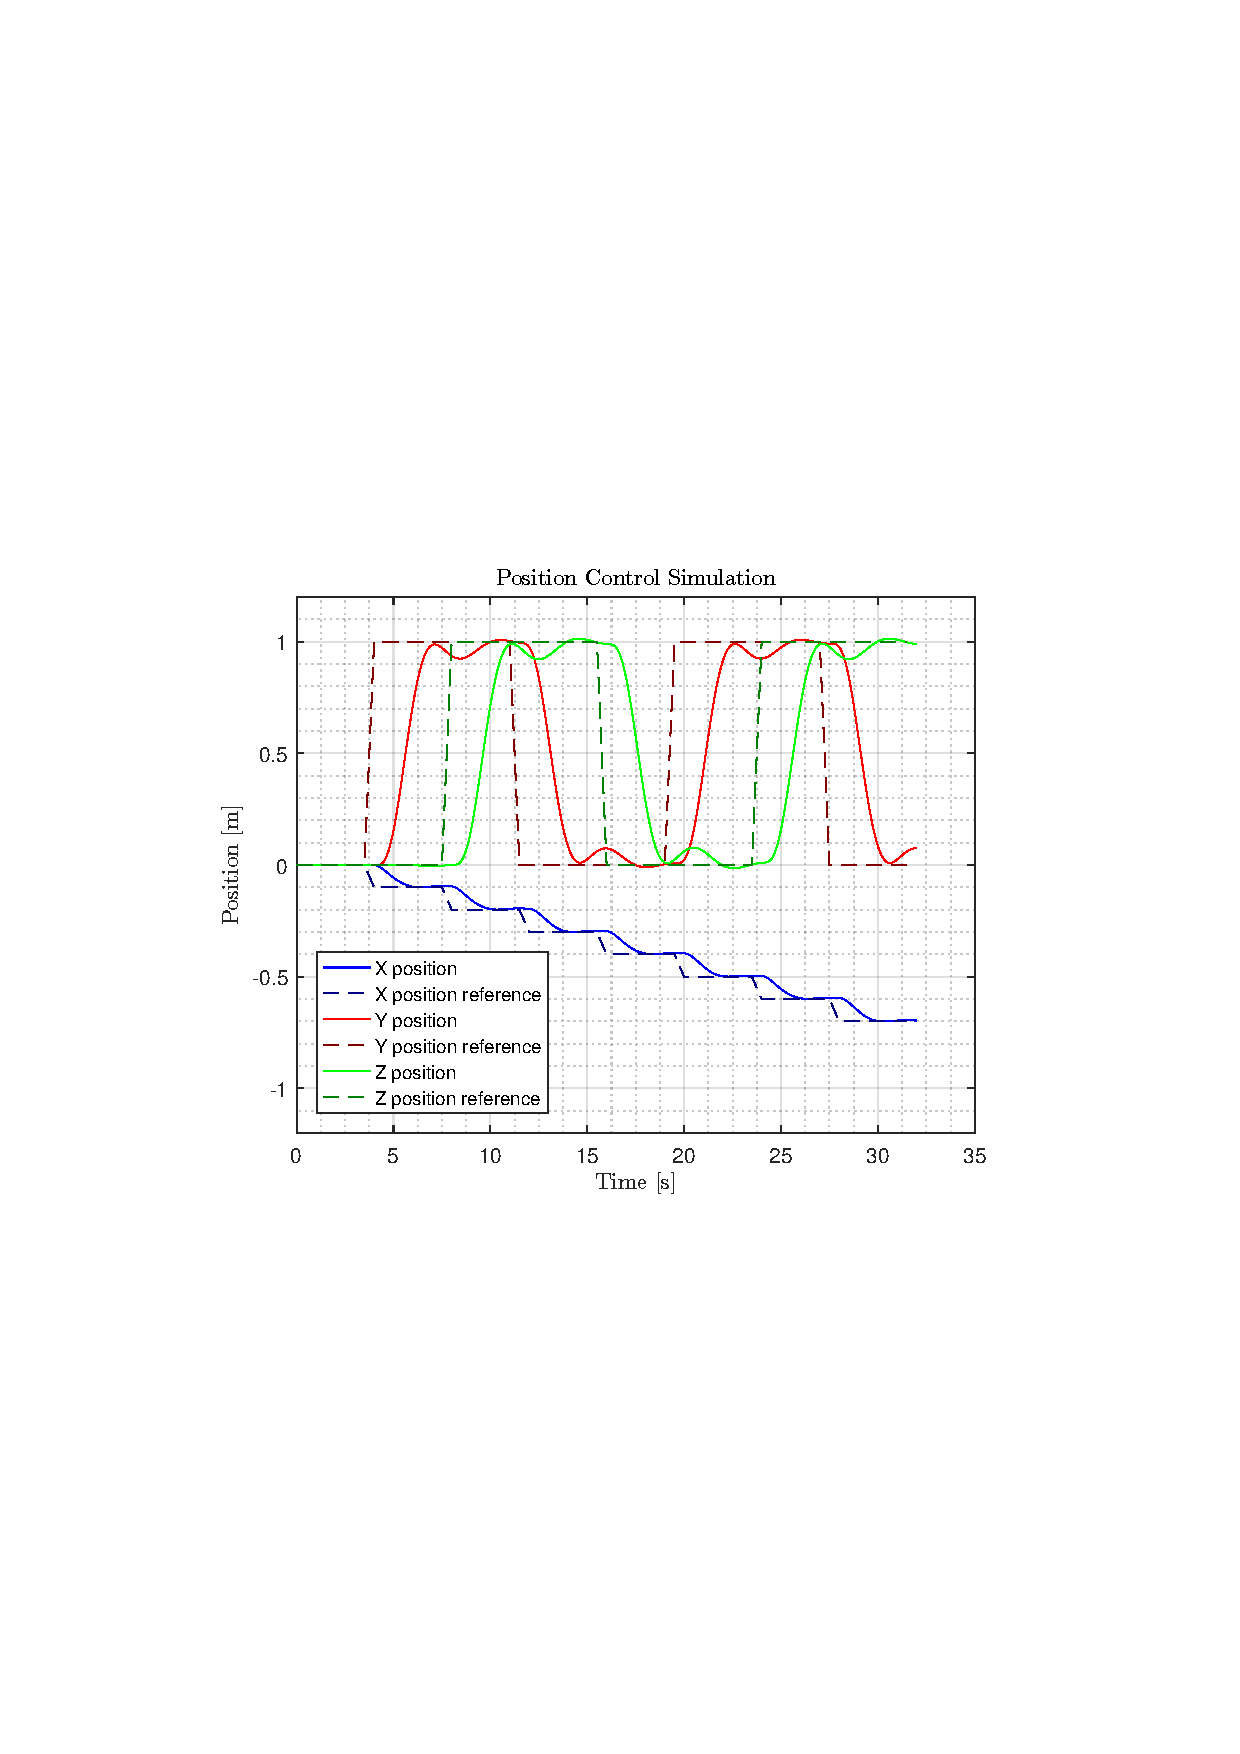
\includegraphics[width=.45\textwidth]{figures/PositionControl}
	\caption{Position control results in the three inertial axes directions. The references given to the control system are shown with dashed lines.}
	\label{PositionControl}
\end{figure}

The inner attitude controller results are also included and shown in \autoref{AttitudeControl} so the performance of the attitude control can be evaluated. 
\begin{figure}[H]
	\centering
	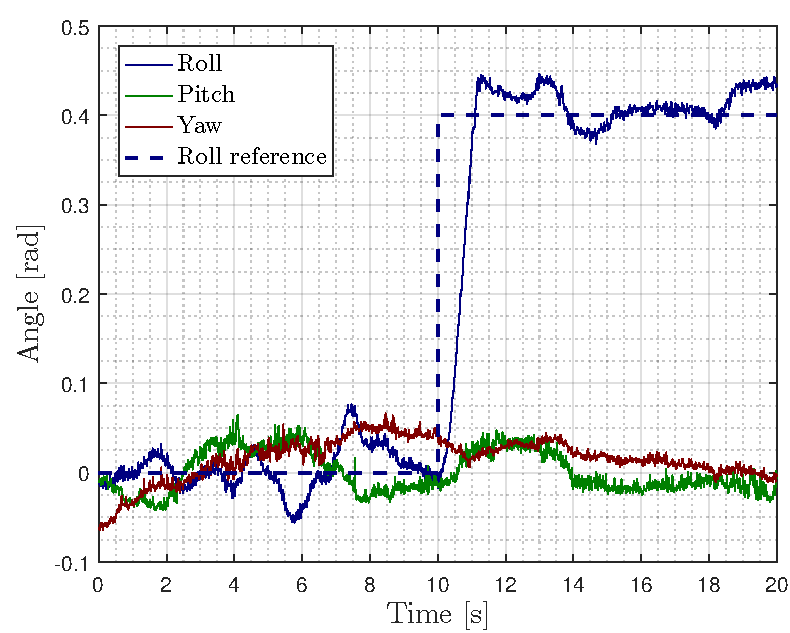
\includegraphics[width=.45\textwidth]{figures/AttitudeControl}
	\caption{Attitude control results in the three angles. The references given to the attitude control system are shown with dashed lines.}
	\label{AttitudeControl}
\end{figure}


